\chapter{Introduction}
\label{Chapter1}

\section{General Background}
Image segmentation is a fundamental task in computer vision that involves partitioning a digital image into multiple segments or sets of pixels, often corresponding to different objects or parts of objects. The goal is to simplify or change the representation of an image into something that is more meaningful and easier to analyze. The history of this field can be broadly divided into three distinct eras.

\textbf{The Pre-Deep Learning Era: Seed-Based and Energy Models}
Before the rise of neural networks, interactive segmentation relied on mathematical frameworks where user inputs acted as "seeds" or constraints for optimization algorithms. These methods focused on low-level features like color gradients and pixel connectivity:
\begin{itemize}
	\item \textbf{Region Growing:} One of the simplest forms of prompt-based segmentation, where a user defines "seed points." The algorithm iteratively clusters neighboring pixels with similar intensity values to the seed, effectively expanding the selection until a boundary is reached \cite{region_growing_2014}.
	\item \textbf{Watershed Transformation:} This method treats an image like a topographic surface. By placing "markers" (prompts) in specific regions, the algorithm simulates flooding from these points, with the boundaries forming where different "water sources" meet \cite{watershed_1979}.
	\item \textbf{Active Contour Models (Snakes):} Introduced by Kass et al. (1988), these are energy-minimizing splines influenced by image forces. A user provides an initial rough contour (a visual prompt), which then "shrinks" or "expands" to fit the edges of the target object \cite{snakes_1988}.
	\item \textbf{GrabCut:} A landmark in interactive segmentation, GrabCut uses a bounding box prompt to initialize a Gaussian Mixture Model. It employs Graph Cuts to iteratively estimate the foreground and background, allowing users to further refine the result with brush strokes \cite{grab_cut_2004}.
\end{itemize}

\textbf{The Deep Learning Era: From Weak Supervision to Interaction}
The integration of Convolutional Neural Networks (CNNs) allowed models to learn semantic context, making visual prompts significantly more powerful and robust to noise.
\begin{itemize}
	\item \textbf{BoxSup and ScribbleSup:} These methods explored using "weak" visual prompts—bounding boxes and scribbles, respectively—as supervision signals. Instead of requiring exhaustive pixel-wise labels for training, these models learned to generate dense masks from simple user-provided annotations \cite{box_sup_2015, scribble_sup_2016}.
	\item \textbf{Deep Extreme Cut (DEXTR):} DEXTR shifted the focus to efficient interaction by requiring only four "extreme points" (top, bottom, left-most, and right-most pixels) of an object. This demonstrated that minimal, precise visual prompts could outperform complex manual segmentation \cite{deep_extreme_cut_2018}.
	\item \textbf{FocalClick:} As interactive segmentation moved toward real-time applications, FocalClick introduced a multi-path design that allows for efficient local refinement. When a user clicks to correct a mask, the model "fuses" the new information locally, significantly reducing the computational overhead of interactive editing \cite{focal_click_2022}.
\end{itemize}

\textbf{The Era of Foundation Models: Segment Anything}
The current state-of-the-art is defined by the shift toward "Foundation Models"—large-scale architectures trained on massive datasets that exhibit zero-shot generalization to unseen objects and domains.
\begin{itemize}
	\item \textbf{Segment Anything Model (SAM):} Developed by Meta AI (2023), SAM introduced the "Promptable Segmentation Task." It is designed to return a valid segmentation mask given any prompt, such as points, bounding boxes, or even text. Trained on the SA-1B dataset of over 1.1 billion masks, SAM can segment any object in any image without prior training on that specific category \cite{kirillov2023segment}.
\end{itemize}

\section{Motivation}
The drive to advance image segmentation stems from both scientific inquiry and practical necessity.

Scientifically, segmentation addresses a fundamental question in perception: while image classification tells us \textit{what} is in an image, segmentation answers \textit{where} it is, down to the pixel level. This granular understanding is crucial for emulating the human ability to parse a scene into distinct objects and regions, forming the basis for true visual comprehension.

Practically, segmentation is an enabling technology for a multitude of real-world applications:
\begin{itemize}
	\item \textbf{Autonomous Driving:} Segmenting lanes, pedestrians, vehicles, and traffic signs is critical for safe navigation.
	\item \textbf{Medical Imaging:} Precise segmentation of tumors, organs, and other anatomical structures is vital for diagnosis, treatment planning, and surgical guidance.
	\item \textbf{Real-World Data Complexity:} Segmentation provides a robust way to handle complex scenes with occluded or overlapping objects.
	\item \textbf{Downstream Vision Tasks:} It serves as a foundational step for numerous other tasks, including object detection, tracking, and detailed semantic scene understanding. Without accurate segmentation, the performance of these downstream applications would be severely limited.
\end{itemize}

The motivation behind the \textbf{Segment Anything Model (SAM)} represents a culmination of these goals. As stated by its creators, ``In this work, our goal is to build a foundation model for image segmentation'' \cite{kirillov2023segment}. The aim was not to create another specialized model but a generalist one. They sought ``to develop a promptable model and pre-train it on a broad dataset using a task that enables powerful generalization. With this model, we aim to solve a range of downstream segmentation problems on new data distributions using prompt engineering'' \cite{kirillov2023segment}. This ambition marks a shift towards creating a single, powerful tool that can handle any segmentation request on any image, democratizing the technology and accelerating research and application development.


\section{Problem Statement}
Image segmentation is the task of grouping pixels that belong to a common semantic object and separating them from other objects and the background. A "semantic object" refers to an entity that is meaningful and recognizable within a given context, such as a car, a person, a tree, or even amorphous regions like "sky" or "road".

The core principle of segmentation is guided by two criteria: pixels within the same group should be as similar as possible, while pixels belonging to different groups should be as distinct as possible. This "similarity" can be defined by various attributes, including color, intensity, texture, or learned semantic features. In essence, the task simulates the human cognitive ability to transform raw, unstructured visual data into a structured representation of distinct entities.

For a modern promptable segmentation system like SAM, the problem can be formally defined by its inputs and outputs.
\begin{itemize}
	\item \textbf{Input:} An image and a "visual prompt" that specifies the object of interest. This prompt can take various forms, such as a point (or multiple points) on the object, a bounding box enclosing it, or even a rough mask.
	\item \textbf{Output:} One or more segmentation masks for the object(s) indicated by the prompt, along with a confidence score for each mask. The ability to output multiple masks is crucial for handling ambiguity (e.g., a single point on a shirt could refer to the shirt or the person wearing it).
\end{itemize}

The general framework for such a system, as shown in Fig. \ref{fig:framework}, typically consists of two main stages: a powerful visual encoder that processes the input image to create a high-dimensional feature representation, and a lightweight decoder that takes this representation along with an encoded prompt to rapidly generate the final mask.

\begin{figure}[t]
	\centering
	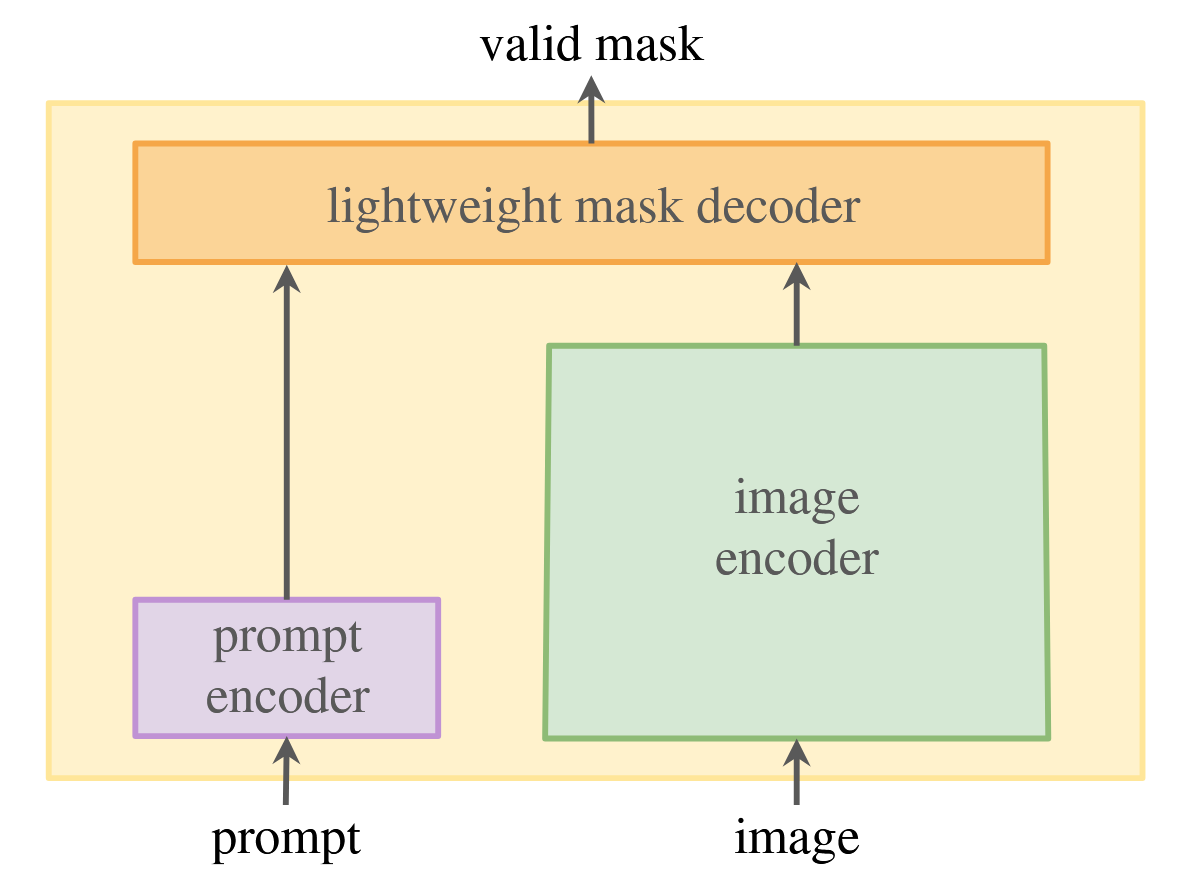
\includegraphics[width=0.7\linewidth]{framework.png}
	\caption{A general framework for a promptable segmentation model. An image encoder computes a feature embedding for the input image. A prompt encoder embeds the user's prompt (e.g., points, boxes). A lightweight mask decoder combines these embeddings to predict segmentation masks in real-time.}
	\label{fig:framework}
\end{figure}


\begin{figure}[t]
	\centering
	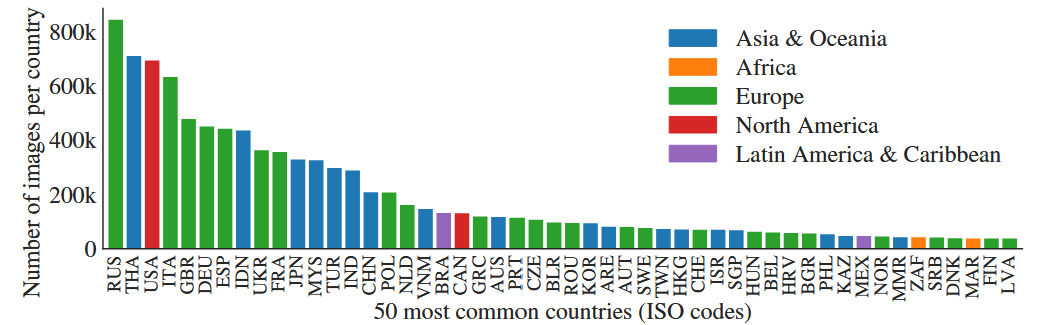
\includegraphics[width=\linewidth]{geo_dist.png}
	\caption{Estimated geographic distribution of SA-1B images. The map shows that most countries are represented with over 1000 images, making it one of the most geographically diverse datasets for computer vision. (Source: \cite{kirillov2023segment})}
	\label{fig:geo_dist}
\end{figure}
%\begin{figure}[H]
%	\centering
%	
\includegraphics{fig1.png} % Replace with your desired image and size
%	\caption{Diagram for Input/ Output here + Framework etc etc} % Add a caption
%%	\label{fig:lorem1} % Label for referencing
%\end{figure}
%% Table 1: Papers, Mechanics, and Methodology
%\begin{table*}[t]
%	%	\centering
%	
%	\begin{center} % maximum 0.75
%		\caption{Comparison Table - Part 1: Methodology}
%		\begin{tabular}{|>{\centering\arraybackslash}p{0.15\textwidth}|>{\centering\arraybackslash}p{0.15\textwidth}|>{\centering\arraybackslash}p{0.15\textwidth}|>{\centering\arraybackslash}p{0.15\textwidth}|>{\centering\arraybackslash}p{0.15\textwidth}|}
%			\hline
%			\multirow{2}{*}{\textbf{Papers}} & 
%			\multirow{2}{*}{\textbf{Mechanics}} & 
%			\multicolumn{3}{c|}{\textbf{Methodology}} \\
%			\cline{3-5} 
%			& &
%			\textbf{\centering\textit{Stage 1}} & 
%			\textbf{\textit{Stage 2}} & 
%			\textbf{\textit{Stage 3}} \\
%			\hline
%			copy copy copy copy copy copy copy copy copy copy copy copy copy copy copy copy \par copy copy copy copy copy copy copy copy & More table copy$^{\mathrm{a}}$ & & & \\
%			\hline
%			\multicolumn{5}{l}{$^{\mathrm{a}}$Sample of a Table footnote.}
%		\end{tabular}
%		\label{tab1}
%	\end{center}
%\end{table*}
%% Table 2: Papers, Performance, Contribution, and Limitation
%\begin{table*}[t!]
%	\caption{Comparison Table - Part 2: Performance and Analysis}
%	\begin{center}
%		\begin{tabular}{|>{\centering\arraybackslash}p{0.125\textwidth}|>{\centering\arraybackslash}p{0.125\textwidth}|>{\centering\arraybackslash}p{0.125\textwidth}|>{\centering\arraybackslash}p{0.125\textwidth}|>{\centering\arraybackslash}p{0.125\textwidth}|>{\centering\arraybackslash}p{0.125\textwidth}|}
%			\hline
%			\multirow{2}{*}{\textbf{Papers}} & 
%			\multicolumn{3}{c|}{\textbf{Performance}} &
%			\multirow{2}{*}{\textbf{Contribution}} & 
%			\multirow{2}{*}{\textbf{Limitation}} \\
%			\cline{2-4}
%			&
%			\textbf{\textit{Data}} & 
%			\textbf{\textit{Metric}} &
%			\textbf{\textit{Result}} &
%			& \\
%			\hline
%			copy & & & & & \\
%			\hline
%			\multicolumn{6}{l}{$^{\mathrm{a}}$Sample of a Table footnote.}
%		\end{tabular}
%		\label{tab2}
%	\end{center}
%\end{table*}


\section{Contribution}
The work on the Segment Anything Model (SAM) introduced several pivotal contributions to the field. As summarized by the authors, ``Our principal contributions are a new task (promptable segmentation), foundational model for that new task (SAM), and dataset (SA-1B) that make this leap possible'' \cite{kirillov2023segment}.

A key contribution is the \textbf{SA-1B dataset}, which remains the largest segmentation dataset to date. Its key features include:
\begin{itemize}
	\item \textbf{Scale:} It contains over 11 million high-resolution images and 1.1 billion high-quality segmentation masks.
	\item \textbf{Privacy-First:} All images are privacy-respecting, with automated blurring of faces and license plates.
	\item \textbf{Diversity:} The dataset is geographically diverse, with a significant number of images from countries around the world, as illustrated in Fig. \ref{fig:geo_dist}. This helps mitigate geographical bias often present in large-scale datasets.
\end{itemize}

The contribution of this report is to provide a comprehensive survey and structured analysis of the field of image segmentation. We synthesize the historical evolution, explain the motivations driving modern research, and offer a detailed examination of the methodology behind foundation models like SAM, contextualizing their impact and outlining future directions.
